
\documentclass{jtetiproposalskripsi}

%-----------------------------------------------------------------
%Disini awal masukan untuk data proposal skripsi
%-----------------------------------------------------------------
\titleind{APLIKASI PENGOBATAN PASIEN BERBASIS SMS GATEWAY}
\fullname{AWALIA WAHYU J}

\idnum{1200631030}

\approvaldate{20 Desember 2014}

\degree{Sarjana Teknik Informatika}

\yearsubmit{2014}

\program{Manajemen Infomatika}

\headprogram{Bagus Setya, S.T., M.T., Ph.D.}

\firstsupervisor{Bahtyar Hadi, S.T., M.Eng.}
\firstnip{1976 0501 2002 12 1 002}

\secondsupervisor{Triawan Adi C, S.T., M.Eng.}
\secondnip{1977 0131 2002 12 1 003}


%-----------------------------------------------------------------
%Disini akhir masukan untuk data proposal skripsi
%-----------------------------------------------------------------

\begin{document}

\cover

\approvalpage

%-----------------------------------------------------------------
%Disini akhir masukan untuk muka skripsi
%-----------------------------------------------------------------

%-----------------------------------------------------------------
%Disini awal masukan Intisari
%-----------------------------------------------------------------
\begin{abstractind}
Rumah Sakit Paru Jember merupakan sasaran utama bagi para pasien yang menderita sakit paru dan gangguan pernafasan. Permasalahan yang dihadapi saat ini adalah banyaknya pasien yang berobat pada rumah sakit ini dan rumah sakit ini belum mempunyai sistem informasi yang berhubungan langsung dengan pasien.

Dengan menggunakan perangkat lunak Java,  MySQL, Gammu, dan Modem GSM sebagai media untuk penyebaran informasi kepada pasien penulis bertujuan untuk mengembangkan informasi di Rumah Sakit Paru Jember ke sisitem penyebaran informasi berbasis SMS Gateway.

Objek utama sistem ini adalah agar pasien yang telah berobat ke Rumah Sakit Paru Jember, nantinya setelah pulang mendapat informasi dan memudahkan pihak Rumah Sakit dalam penyebaran informasi serta kecepatan dalam pengiriman informasi. Dan melalui sistem SMS Gateway ini akhirnya dapat meningkatkan layanan Rumah Sakit kepada para pasien.


\bigskip
\textbf{Kata kunci} : Sistem Informasi, Penjadwalan.
\end{abstractind}
%-----------------------------------------------------------------
%Disini akhir masukan Intisari
%-----------------------------------------------------------------

\tableofcontents
\addcontentsline{toc}{chapter}{DAFTAR ISI}
\selectlanguage{bahasa}\clearpage\pagenumbering{arabic}\setcounter{page}{1}

%-----------------------------------------------------------------
%Disini awal masukan untuk Bab
%-----------------------------------------------------------------
\chapter{LATAR BELAKANG}

\section{Latar Belakang Masalah}
Perkembangan teknologi telah banyak digunakan dalam kegiatan sehari-hari di kalangan masyarakat, khususnya di rumah sakit. Rumah Sakit Paru Jember sangat berperan penting dalam proses penyembuhan pasien. Karena setiap pasien yang sakit sangat menginginkan cepat sembuh.

Seiring dengan perkrmbangan teknologi, maka dibutuhkan sebuah aplikasi untuk menyebarkan informasi secara mudah, cepat, dan akurat. Contohnya dalam penyebaran informasi kepada para pasiennya. di Rumah Sakit Paru Jember ini proses penyebaran informasi masih menggunakan cara manual, misalnya masih menggunakan cara lisan dalam mengigatkan para pasien yang telah datang berobat dan memberi tahu secara lesan jadwal kembali kontrol. Tentunya cara tersebut  memiliki kekurangan dalam hal waktu dan mudah dilupakan oleh pasien. Oleh karena itu dibutuhkan seuah aplikasi khusus untuk penyebaran informasi tersebut.

Berdasarkan uraian diatas maka sms gateway merupakan  suatu solusi untuk menanggulangi masalah-masalah dalam penyebaran informasi. Oleh karena itu penulis mengambil judul \textbf{Aplikasi Pengobatan pasien Berbasis SMS Gateway}. Didalam aplikasi ini, karyawan yang mrnjadi administrator nantinya dapat mmenyebarkan informasi kepada para psien secara  cepat dan mudah.


\section{Rumusan Masalah}
Berdasarkan uraian yang telah dipaparkan sebelumnya, maka dapat dirumuskan permasalahan yakni :
\begin{itemize}
\item[1.]	Bagaimana penyebaran informasi secara cepat dan akurat.
\item[2.]	Bagaimana penerapan smsm gateway terhadap penyebaran informasi.
\end{itemize}



\section{Batasan Masalah}
Beberapa batasan masalah dalam penelitian ini adalah :
\begin{itemize}
\item[1.]	Sms hanya berupa pesan teks.
\item[2.]	Aplikasi ini masih terbatas pengiriman informasi hanya kepada pasien.
\item[3.]	Aplikasi ini hanya berjalan pada aplikasi windows.
\end{itemize}

\section{Tujuan Penelitian}
Tujuan dari dibuatnya aplikasi ini adalah untuk memudahkan proses penyebaran informasi kepada pasien serta pengiriman informasi yang cepat dan akurat.


\section{Manfaat Penelitian}
Manfaat yang diperoleh dari penggunaan aplikasi ini bagi rumah sakit, dan khususnya yang menggunakan aplikasi ini adalah kemudahan dalam penyebaran informasi dan kecepatan dalam pengiriman iformasi.
Sehingga para pasien yang sudah datang berobat dan setelah pulang mendapat informasi tentang jadwal kontrol pasien.


%-------------------------------------------------------------------------------
\chapter{LANDASAN TEORI}                

\section{Landasan Teori}
\subsection{Sistem}
Terdapat dua kelompok pendekatan di dalam pendefinisian sistem, yaitu kelompok yang menekankan pada prosedur dan kelompok yang menekankan pada elemen atau komponennya. Pendekatan yang menekankan pada prosedur mendefinisikan sistem sebagai suatu jaringan kerja dari prosedur-prosedur yang saling berhubungan. Sedangkan pendekatan sistem yang lebih menekankan pada elemen atau komponen mendefinisikan sistem sebagai kumpulan dari elemen-elemen yang berinteraksi untuk mencapai suatu tujuan tertentu. Kedua kelompok definisi ini adalah benar dan tidak bertentangan, yang berbeda adalah cara pendekatannya saja.
\\

Secara sederhana sistem dapat diartikan sebagai suatu kumpulan atau himpunan dari unsur, komponen atau variabel-variabel yang terorganisasi, saling berinteraksi, saling tergantung satu sama lain dan terpadu.
\\

Sistem adalah kelompok elemen yang terintegrasi dengan maksud yang sama untuk mencapai suatu tujuan. (McLeod dalam Ladjamudin bin Al-Bahra, 2005)
Pendekatan sistem yang lebih menekankan pada prosedur didefinisikan bahwa sistem yaitu suatu jaringan kerja dari prosedur-prosedur yang saling berhubungan, berkumpul bersama-sama untuk melakukan suatu kegiatan atau menyelesaikan suatu sasaran tertentu. (Gerald.J.1991 dalam Ladjamudin bin Al-Bahra,2005)
\\

Dengan demikian definisi ini akan mempunyai peranan yang sangat penting dalam melakukan pendekatan terhadap sistem yang dianalisis. Pendekatan sistem dari kumpulan komponen atau elemen-elemen atau subsistem-subsistem lebih luas dibandingkan pendekatan sistem yang lebih menekankan pada prosedurnya. Karena pendekatan sistem yang lebih menekankan pada komponen akan lebih mudah dipelajari untuk analisis dan rancangan system. 
           ( Sumber : Ladjamudin, bin Al-Bahra, 2005, Analisis dan Desain Sistem Informasi).

\subsection{Informasi}
Informasi adalah sebagai data yang telah diolah menjadi bentuk yang lebih berarti dan berguna bagi penerimanya untuk mengambil keputusan masa kini maupun masa yang akan datang. (Gordon.B.Davis (1985) dalam Ladjamudin, bin Al-Bahra, 2005).
\\

Sumber informasi adalah data. Data adalah kenyataan yang menggambarkan kejadian-kejadian yang diperoleh setelah data-data mentah diproses dan diolah 
\\

Menurut John Burch dan Gary Grudnitski, agar informasi dihasilkan lebih berharga, maka informasi harus memenuhi kriteria sebagai berikut :
\begin{itemize}

\item[1.]	Informasi harus akurat, sehingga mendukung pihak manajemen dalam mengambil keputusan.
\item[2.]	Informasi harus relevan, benar-benar terasa manfaatnya bagi yang membutuhkan.
\item[3.]	Informasi harus tepat waktu, sehingga tidak ada keterlambatan pada saat dibutuhkan.
\end{itemize}

\subsection{Sistem Informasi}
Sistem Informasi dapat didefinisikan sebagai berikut :
\begin{itemize}

\item[a.]	Suatu sistem yang dibuat oleh manusia yang terdiri dari komponen-komponen dalam organisasi untuk mencapai suatu tujuan yaitu menyajikan informasi.
\item[b.]	Sekumpulan prosedur organisasi yang pada saat dilaksanakan akan memberikan informasi bagi pengambil keputusan atau untuk mengendalikan organisasi.
\end{itemize}

\subsection{Database}
Database Management System (DBMS) berisi satu koleksi data yang saling berelasi dan satu set program untuk mengakses data tersebut. Jadi DBMS terdiri dari database dan set program pengelola untuk menambah data, menghapus data, mengambil dan membaca data.

\subsubsection{Definisi Basis Data}
Basis data adalah kumpulan file-file yang mempunyai kaitan antara satu file dengan file yang lain sehingga membentuk satu bangunan data untuk menginformasikan satu perusahaan, instansi dealam batasan tertentu.

\subsubsection{Kegunaan basis Data}
Penyusunan suatu basis data digunakan untuk mangatasi masalah-masalah pada penyusunan data, yaitu :
\begin{itemize}

\item[1.]	Redudansi dan inkonsistensi data
Penyimpanan data yang berulang-ulang di beberapa file dapat mengakibatkan juga inkonsistensi (tidak konsisten) pada data. Untuk itulah diperlukan basis data untuk meng-update data sewaktu-waktu jika terjadi perubahan.
\item[2.]	Kesulitan pengaksesan data
Dengan adanya DBMS yang mampu mengambil data secara langsung dengan bahasa yang familiar dan mudah digunakan (user friendly, maka kesulitan untuk mangakses data yang diinginkan tidak akan terjadi.
\item[3.]	Isolasi data untuk standarisasi
Jika data tersebar dalam beberapa file dalam bentuk format yang tidak sama, maka ini menyulitkan dalam menulis program aplikasi untuk mengambil dan menyimpan data. Maka haruslah data dalam satu database dibuat satu format sehingga mudah dibuat program aplikasinya.
\item[4.]	Multiple user (banyak pemakai)
Dengan adanya basis data, maka dapat diakses pada program yang sama atau digunakan oleh banyak pemakai dalam waktu yang berbeda.
\item[5.]	Masalah keamanan (security)
Tidak setiap pemakai sistem basis data diperbolehkan untuk mengakses semua data. Keamanan data ini dapat diatur lewat program yang dibuat oleh pemrogram atau fasilitas keamanan dari sistem operasi.
\item[6.]	Masalah integrasi (kesatuan)
Database berisi file-file yang saling berkaitan, masalah utama adalah bagaimana kaitan antara file tersebut terjadi. Misalnya file A berkaitan dengan file B, namun secara teknis maka ada kunci yang mengaitkan kedua file tersebut.
\item[7.]	Masalah data independence (kebebasan data)
Pembuatan suatu program aplikasi tidak bebas terhadap database yang ada.
\end{itemize}


\section{SMS (Short Message Service)}
SMS adalah protokol telekomunikasi yang membantu kita mengirimkan pesan pendek (Sebanyak 160 karakter) berupa karakter alfanumerik. SMS merupakan layanan komplementer dari 2 layanan sistem utama jaringan nirkabel digital, baik GSM (Global System for Mobile Communication) maupun CDMA (Code Division Multiple Access), yakni layanan voice dan switched data.

\subsection{SMS Gateway}
Sms Gateway merupakan sebuah perangkat yang menawarkan layanan pengiriman pesan ke jaringan selular dari media lain, atau sebaliknya, sehingga memungkinkan pengiriman atau penerimaan pesan dengan atau tanpa menggunakan ponsel. Sma gateway dapat terhubung ke media lain seperti perangkat link IP untuk memproses suatu layanan SMS. Sebuah sistem SMS (Server/komputer yang dilengkapi dengan perangkat jaringan) dan software (Aplikasi yang digunakan untuk pengolahan pesan). Dan untuk sebuah sistem yang besar umunya dapat menggunakan database untuk penyimpanan data.

%-------------------------------------------------------------------------------
\chapter{METODE PENELITIAN}

\section{Flowchart Metode Penelitian}
\begin{figure}[ht!]
\centering
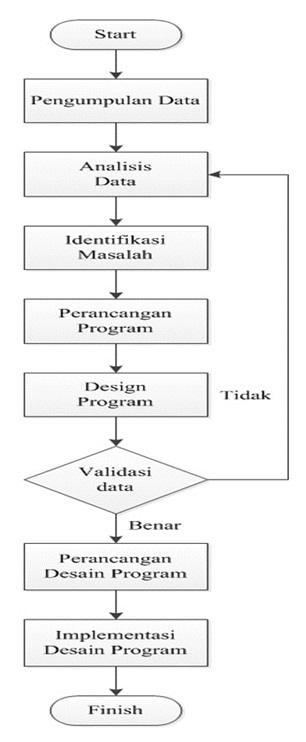
\includegraphics[width=0.4\textwidth]{gambar/flowchart}
\caption{Flowchart Metode Penelitian}
\label{wsn}
\end{figure}
\newpage
Secara garis besar alur sistem informasi yang dibuat dapat digambarkan dengan flowchart sistem seperti diatas.
\begin{itemize}

\item	Penelitian dimulai dengan mengumpulkan data dari sumber yang terlibat langsung dari penelitian yang berupa wawancara dan quisioner. 
\item	Setelah data sudah lengkap maka data tersebut dianalisis yang ditujukan untuk mengelompokkan data yang berasal dari wawancara dan quisioner. Kedua proses tersebut dilakukan secara manual karena proses pengambilan data diambil langsung dari Rumah Sakit. 
\item	Setelah semua data terkumpul barulah dilakukan identifikasi masalah yang ada pada sistem lama.
\item	Setelah itu merancang sistem baru yang akan dibuat perancangan program di Rumah Sakit Paru Jember.
\item	Setelah program terancang, maka dilakukan desain yaitu dengan cara merancang bagaimana program tersebut akan dibuat.
\item	Apabila masih ada kekurangan dari sistem yang lama maka proses tersebut akan berulang mulai dari analisis data. 
\item	Apabila tidak ada validasi data maka dilanjutkan dengan perancangan desain program yang sudah dibuat.
\item	Dan apabila sudah memenuhi barulah merancang desain sistem baru yang disesuaikan dengan semua data yang sudah diperoleh dan mengimplementasi desain tersebut.
\end{itemize}



\section{Jenis dan Sumber Data}
Jenis dan sumber data yang digunakan dalam pembuatan penelitian ini adalah menggunakan jenis data yaitu data primer dan data sekunder.

\subsection{Data Primer}
Data primer adalah data yang dikumpulkan, diolah dan disajikan oleh penulis berdasarkan data sekunder. Berbagai data primer yang dihasilkan meliputi data laporan pasien yang datang berobat.

\subsection{Data Sekunder}
Data yang diperoleh dari tempat penelitian dengan mengumpulkan data berupa dokumen-dokumen yang berkaitan dengan pasien yang datang berobat.

\section{Metode Pengumpulan Data}
Berikut beberapa metode yang digunakan penulis untuk memperoleh data, sebagai berikut :
\begin{itemize}

\item[a.]	Wawancara
 \\
 Adalah metode pengumpulan data dengan jalan tanya jawab seperti yang dilakukan secara sistematik dan berdasarkan pada tujuan penelitian yang dilakukan.
\item[b.]	Studi Pustaka
 \\
 Adalah metode yang menggunakan buku literatur untuk mendapatkan tujuan teoritis sebagai dasar untuk melakukan analisis terhadap system.
\item[c.]	Observasi
\\
Merupakan cara untuk mendapatkan data dan informasi dengan melakukan peninjauan atau pengamatan secara langsung ketempat yang berkaitan dengan penulisan Tugas Akhir dan pembuatan sistem informasinya.
\end{itemize}

\section{Alat Bantu}
Dalam melakukan penelitian ini, ada alat bantu dalam proses pengerjaannya, yaitu :

\subsection{Perangkat Keras}
\begin{itemize}

\item[a.]	Prosessor amd
\item[b.]	Memori 2 GB
\item[c.]	Harddisk 500 GB
\end{itemize}

\subsection{Perangkat Lunak}
\begin{itemize}

\item[a.]	Sistem Operasi Microsoft Windows 7
\item[b.]	Adobe Dreamweaver
\item[c.]	Java
\item[d.]	MySQL

\end{itemize}

\section{Jadwal Penelitian}
Dalam pengerjaan laporan ini agar penelitian tersebut dapat diselesaikan sesuai dengan waktu yang sudah direncanakan maka peneliti membuat suatu jadwal penelitian berupa jadwal matrik untuk tahapan jadwal, yaitu :
\begin{table}[ht!]
\centering
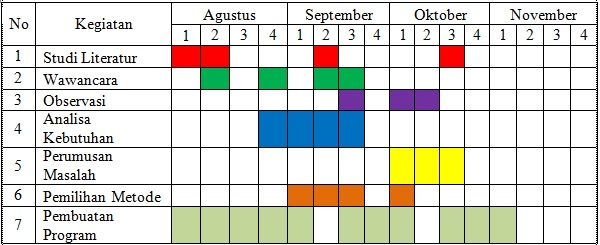
\includegraphics[width=1\textwidth]{gambar/jadwal}
\caption{Jadwal Penelitian}
\label{wsn}
\end{table}
\newpage

\end{document}